\section{»Dinge«, Referenzen und Pointer}


\subsection{»Dinge« und Speicher}

\begin{frame}[fragile]{»Dinge«}
	Das grundlegende Konzept in C++ nennt sich im Standard \enquote{object}. Hinsichtlich Java und Objektorientierung aber missverständlich!
	Wir nennen es daher »Ding«.
	
	\pause
	\vspace{2em}
	
	{\footnotesize
	\begin{block}{Ein Beispiel}
		\lstinputlisting[language=C++, linerange={3-3}]{cpp-code/objects.cpp}
		Es gibt jetzt ein »Ding« mit dem Namen \verb|foo| und dem Typen \verb|int|.
	\end{block}
	}
\end{frame}

\begin{frame}[fragile]{Definition: »Ding«}
	\begin{block}{Standard, 1.8}
		Ein »Ding«
		\begin{enumerate}
			\item<1-| alert@1> ist ein Speicherbereich, aber \emph{keine} Funktion {\tiny(auch wenn diese Speicher belegt!)}.
			\item<2-| alert@2> hat eine Speicherdauer, einen Typen und \emph{kann} einen \emph{Namen} haben.
			% der Rest soll übersprungen werden und ist als Referenz gedacht
			\item<3-> {\footnotesize hat eine Größe von einem oder mehr Bytes {\tiny (abgesehen von bit-fields)}.}
			\item<3-> {\footnotesize von »einfachem« {\tiny (POD)} Typ besetzt eine zusammenhängende Menge Bytes.}
			\item<3-> {\footnotesize wird durch eine Definition, den \verb|new|-Ausdruck oder vom Compiler erzeugt.}
		\end{enumerate}
	\end{block}
\end{frame}

\begin{frame}{Speicher}
	\begin{block}{Standard, 1.7}
		\begin{itemize}[<+->]
			\item Die fundamentale Speicher-Einheit im C++ Speichermodell ist das \emph{Byte}.
			\item Was ein Byte ist, ist recht abstrakt definiert.
			\item Der Speicher, welcher einem C++ Programm zur Verfügung steht, besteht aus einer oder mehreren Sequenzen von zusammenhängenden Bytes.
			\item Jedes Byte hat eine eindeutige Adresse.
		\end{itemize}
	\end{block}
	
	\uncover<+->
	{
		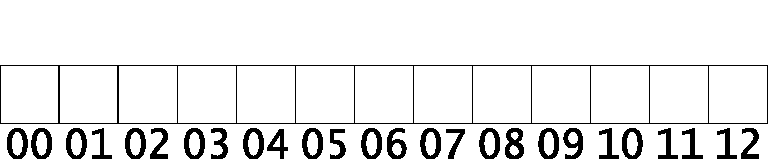
\includegraphics[width=\linewidth]{images/free}
	}
\end{frame}

\begin{frame}[fragile]{»Dinge« und Speicher}
	Ein »Ding« ist ein Speicherbereich. Wie hängt dieser Speicherbereich mit dem Speicher zusammen, der meinem Programm zur Verfügung steht?\\
	
	\pause
	
	\begin{block}{Beispiel: Ein paar »Dinge«}
		Am einfachsten legt man »Dinge« mittels einer  Definitionen an.\\
		{\tiny Ausnahme: \verb|static|}
		
		{\footnotesize
		\begin{block}{}
			\lstinputlisting[language=C++, linerange={3-4, 6-6}]{cpp-code/objects.cpp}
		\end{block}
		}
		
		\pause
		
		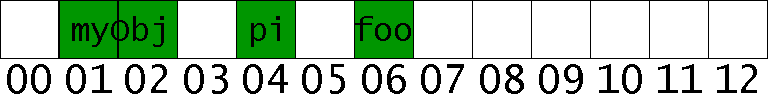
\includegraphics[width=\linewidth]{images/object_things}
	\end{block}
\end{frame}


\subsection{Referenzen}

\begin{frame}[fragile]{»Dinge« und Referenzen}
	Eine Referenz ist ein zusätzlicher Namen für \emph{dasselbe} »Ding«.\\
	Die Speicherdauer wird dadurch \emph{nicht} beeinflusst.
	
	{\footnotesize
	\begin{block}{}
		\lstinputlisting[language=C++, linerange=16-17]{cpp-code/objects.cpp}
	\end{block}
	}
	
	\pause
	
	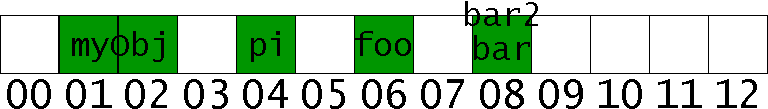
\includegraphics[width=\linewidth]{images/object_refs}
	
	\pause
	
	{\footnotesize
	\begin{block}{}
		\lstinputlisting[language=C++, linerange=14-15]{cpp-code/objects.cpp}
	\end{block}
	}
\end{frame}

{\refframe
\begin{frame}[fragile]{Referenz: Referenzen}
	\verb|TYPE& addName = origName;|
	\begin{itemize}
		\item Führt \verb|addName| als zusätzlichen Namen für das »Ding« mit dem Namen \verb|origName| ein.
		\item \verb|addName| heißt auch eine Referenz auf \verb|origName|.
	\end{itemize}
	
	\vspace{2em}
	
	Achtung: Eine Referenz muss immer gleich »initialisiert« werden, d.h. mittels \verb|=| einem »Ding« zugeordnet. {\tiny Bei Klassen-Membern in der Initialisations-Liste des Konstruktors.}
\end{frame}
}

\begin{frame}[fragile]{Referenzen als Parameter}
	Nutzt man eine Referenz als Parameter, so kann man innerhalb der Funktion den Wert des übergebenen »Dings« ändern:
	
	{\footnotesize
	\begin{block}{}
		\lstinputlisting[language=C++, linerange=34-38]{cpp-code/objects.cpp}
	\end{block}
	}
	
	\pause
	
	{\footnotesize
	\begin{block}{}
		\lstinputlisting[language=C++, linerange=19-22]{cpp-code/objects.cpp}
	\end{block}
	}
\end{frame}


\subsection{Pointer}

\begin{frame}[fragile]{Adressen und Pointer}
	\begin{itemize}[<+->]
		\item Jedes Byte hat eine eindeutige Adresse.
		\item Man darf keine Annahmen darüber treffen, wie diese Adresse tatsächlich aussieht oder wie groß sie ist!
		\item Was man tun darf, sind Operationen mit \emph{Pointern}.
		\item Ein Pointer ist ein »Ding«, dessen Inhalt eine Adresse ist.
	\end{itemize}
	
	\uncover<+->
	{
		\vspace{1em}
		
		Wir wollen jedoch zwecks Anschauung eine Adresse mit der Nummer \emph{der} Bytes eines »Dings« identifizieren.
	
		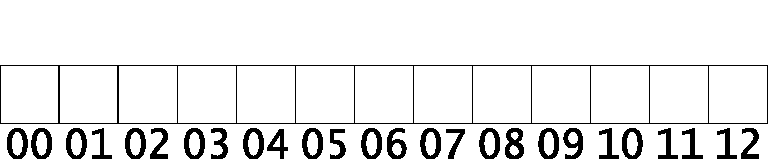
\includegraphics[width=\linewidth]{images/free}
	}
\end{frame}

\begin{frame}[fragile]{»Dinge« und Pointer}
	Sei \verb|NAME| der Name eines »Dings«. Mit \verb|&NAME| erhalte ich dann die Adresse des »Dings«, und zwar in der Form eines Pointers.
	
	\vspace{1em}
	\pause
	
	Als »Ding« hat der Pointer einen Typ:
	{\footnotesize
	\begin{block}{}
		\lstinputlisting[language=C++, linerange=24-25]{cpp-code/objects.cpp}
	\end{block}
	}
	
	\pause
	
	Das »Ding« \verb|NAME| habe den Typen \verb|TYPE|. Dann hat ein Pointer auf das »Ding« den Typ \verb|TYPE*|.
\end{frame}


\begin{frame}[fragile, t]{»Dinge«, Pointer und Adressen}
\begin{overprint}
	\footnotesize
	\begin{block}{Ein Beispiel:}
		\onslide*<1>
		{
			\lstinputlisting[language=C++, linerange={3-4, 6-6}]{cpp-code/objects.cpp}
		}
		\onslide*<2>
		{
			\lstinputlisting[language=C++, linerange={3-4, 6-6, 10-10}]{cpp-code/objects.cpp}
		}
		\onslide*<3->
		{
			\lstinputlisting[language=C++, linerange={3-4, 6-6, 10-10, 27-27}]{cpp-code/objects.cpp}
		}
	\end{block}
	
	\vspace{1em}
	\onslide*<4>
	{
		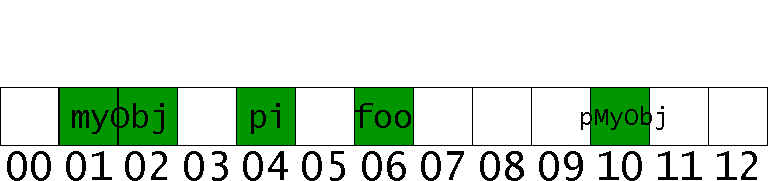
\includegraphics[width=\linewidth]{images/object_points_addr_0}
	}
	\onslide*<5->
	{
		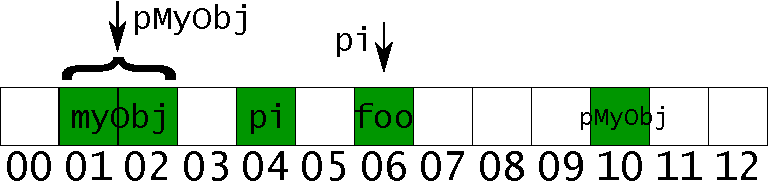
\includegraphics[width=\linewidth]{images/object_points_addr_1}
	}
\end{overprint}
\end{frame}


\begin{frame}[fragile]{Dereferenzieren}
	Wie greife ich auf das »Ding« zu, auf welches ein Pointer verweist?
	
	\vspace{0.5em}
	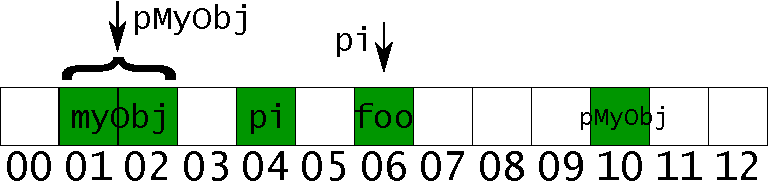
\includegraphics[width=0.75\linewidth]{images/object_points_addr_1}
	\vspace{0.5em}
	
	\pause
	\vspace{1em}
	
	Mittels \verb|*pointerName|. Man kann diesen Ausdruck deuten als:\\
	\emph{das »Ding« an der Adresse, die in} \verb|pointerName| \emph{gespeichert ist}.
	{\footnotesize
	\begin{block}{Beispiel}
		\lstinputlisting[language=C++, linerange=41-42]{cpp-code/objects.cpp}
	\end{block}
	}
\end{frame}


\begin{frame}[fragile]{Pointer vs. Referenzen}
	\footnotesize
	\begin{tabular}{c|c}
		Pointer & Referenz \\ \hline
		ist ein »Ding« & ist nur ein zusätzlicher Name \\
		enthält eine Adresse & enthält selbst nichts \\
		Inhalt kann sich ändern & bezieht sich immer auf dasselbe »Ding« \\
		Inhalt muss nicht sinnvoll sein & bezieht sich auf ein existierendes »Ding« \\
	\end{tabular}
	
	\pause
	
	{\footnotesize
	\begin{block}{}
		\lstinputlisting[language=C++, linerange={4-4, 27-31}]{cpp-code/objects.cpp}
	\end{block}
	}
\end{frame}


\subsection{Arrays}

\begin{frame}[fragile]{Definition eines Arrays}
	Mit \verb|TYPE name[STATIC_NUMBER];| erzeuge ich \verb|STATIC_NUMBER| »Dinge« hintereinander und zusammenhängend.
	
	\pause
	\vspace{1em}
	
	\begin{block}{Beispiel}
		{\footnotesize
			\lstinputlisting[language=C++, linerange={44-44}]{cpp-code/objects.cpp}
		}
	
		\vspace{1em}
		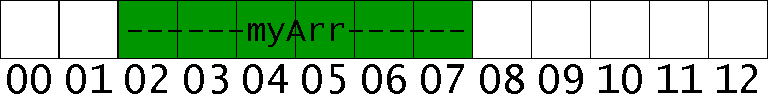
\includegraphics[width=0.75\linewidth]{images/array_small}
	\end{block}
\end{frame}

\begin{frame}[fragile]{Zugriff auf die Elemente}
	Mit \verb|name[DYNAMIC_NUMBER]| greife ich auf ein Element zu, d.h. auf das \verb|DYNAMIC_NUMBER|-te »Ding« im Array.
	
	\vspace{1em}
	\pause
	
	\begin{block}{Beispiel}
		{\footnotesize
			\lstinputlisting[language=C++, linerange={44-45}]{cpp-code/objects.cpp}
		}
	
		\vspace{1em}
		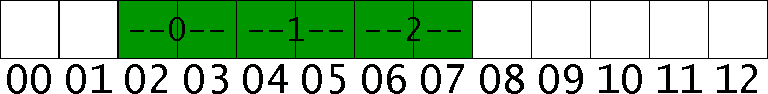
\includegraphics[width=0.75\linewidth]{images/array_elems_small}
	\end{block}
\end{frame}

\begin{frame}[fragile]{Arrays und Pointer}
	\small
	\begin{itemize}[<+->]
		\item Ein »Ding« erzeugt durch \verb|TYPE name[N];| hat den Typen \emph{Array von N TYPEs}.
		\item Ein \emph{Array von N TYPEs} wird automatisch (wo erforderlich) zu einem \verb|TYPE*| konvertiert.
		\item Der so entstehende Pointer zeigt auf \verb|name[0]|.
	\end{itemize}
	
	\uncover<+->
	{
		\begin{block}{Beispiel}
			{\footnotesize
				\lstinputlisting[language=C++, linerange={44-44, 47-48}]{cpp-code/objects.cpp}
			}
			
			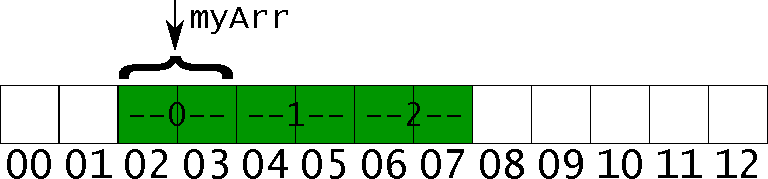
\includegraphics[width=0.75\linewidth]{images/array_elems}
		\end{block}
	}
\end{frame}

\begin{frame}[fragile]{Elemente und Pointer}
	\begin{block}{Beispiel}
		{\footnotesize
			\lstinputlisting[language=C++, linerange={44-44, 47-47}]{cpp-code/objects.cpp}
		}
		
		\onslide<2->
		{
			{\footnotesize
				\lstinputlisting[language=C++, linerange={50-51}]{cpp-code/objects.cpp}
			}
		}
		
		\onslide<3->
		{
			{\footnotesize
				\lstinputlisting[language=C++, linerange={53-54}]{cpp-code/objects.cpp}
			}
		}
		
		\vspace{1em}
		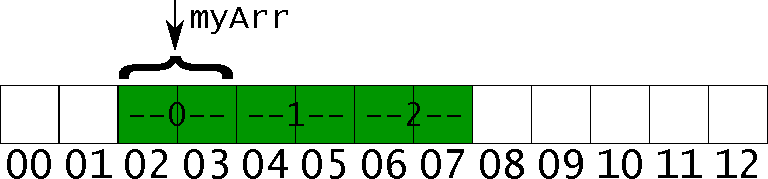
\includegraphics[width=0.75\linewidth]{images/array_elems}
	\end{block}
\end{frame}
